%% \begin{figure}
%% \centering
%% \vspace{-1mm}
%% 	\begin{subfigure}[b]{0.65 \textwidth}
%% 	\begin{footnotesize}
%% 	  1. Consider a replica that has witnessed effects $\{\eta_1,\eta_2,\eta_3\}$.
%%           Suppose an operation $op$ arrives with a \textsf{UB} contract that
%%           requires it to witness effect $\eta_4$  if it	witnesses $\eta_1$, a property
%%           that is mandated by the $\visZ$ relation.\\
%% 	  2. A violation of the contract occurs if $op$ witnesses $\eta_1$ because $\eta_4$
%%           has not yet been seen (left); a ilteration mechanism that \emph{hides} $\eta_1$, however,
%%           allows the contract to be enforced (right).
%% 	\end{footnotesize}
%% 	\end{subfigure}
%% 	~
%% 	\begin{subfigure}[b]{0.298 \textwidth}
%% 	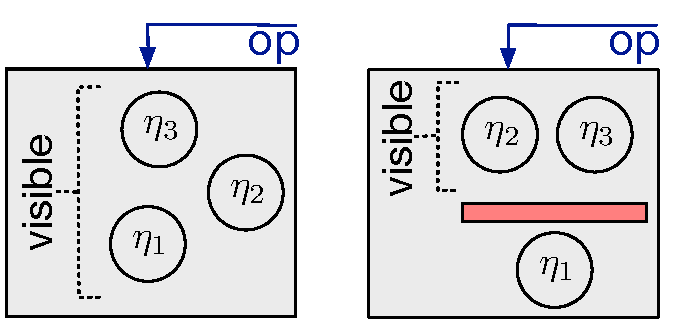
\includegraphics[scale=0.36]{Figures/ub.pdf}
%% 	\end{subfigure}
%% 	\caption{Filtration and \UB{} contracts}
%% \vspace{-5mm}
%% \label{fig:ub}
%% \end{figure}

\begin{figure}
  \centering
  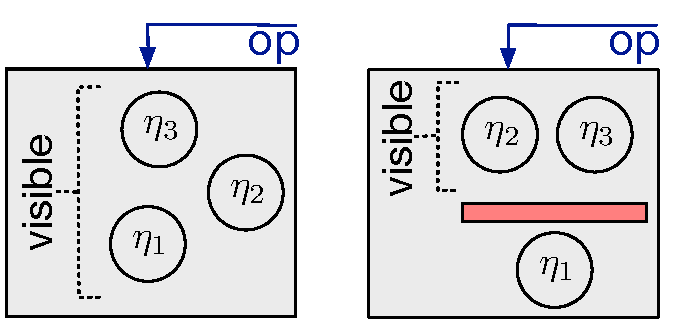
\includegraphics[scale=0.36]{Figures/ub.pdf}
  \caption{\small Filtration and \UB{} contracts.  Consider a replica that
    has witnessed effects $\{\eta_1,\eta_2,\eta_3\}$.  Suppose an
    operation $op$ arrives with a \textsf{UB} contract that requires
    it to witness effect $\eta_4$ if it witnesses $\eta_1$, a property
    that is mandated by the $\visZ$ relation.  . A violation of the
    contract occurs if $op$ witnesses $\eta_1$ because $\eta_4$ has
    not yet been seen (left); a filtration mechanism that \emph{hides}
    $\eta_1$, however, allows the contract to be enforced (right).}
  \label{fig:ub}
\end{figure}  
  
